\section{Goals and Preliminaries}\label{goals}
In this section, we start with an higlight of the macro goals of the thesis, then we expand the content of Section \ref{motivations} by detailing our specific goals and the pheasibilty of each of them. Finally, we summarize the work done in the first year in relation to the proposed goals.

\subsection{Goals}\label{sub_goals}
The high level goals of this thesis are:
\begin{itemize}
    \item To show the relevant role that embeddings can play in searching tasks;
    \item To show that embeddings can be used directly to answer queries instead of beeing an orthogonal part of the answering process.
\end{itemize}

The overall goal of this research proposal is the study of the role of embeddings in data augmentation, from tables augmentation on data lakes to an embedding algorithm for knowledge bases, passing through the integration of embeddings in existing tables augmentation framework exploiting knowledge bases. We organize the work into five main objectives, each leading to specific results. 
The aim of Objective 1 (indexing data lakes to augment) is to analyze the state of the art on open data search, sketching and approximation of information theory measures and to define an index for tables augmentation in data lakes based on information-theoretic measures. 
Objective 2\footnote{Objectives 1 and 2 are developed in parallel} (functional dependencies for augmentation) is aimed at analyzing state of the art on functional dependency discovery algorithms and their links with augmentation. 
The aim of Objective 3 (augmentating via knowledge bases) is to analyze the state of the art approaches in knowledge bases representation and augmentation, along with their role in augmenting tables and integrating of embeddings in such approaches. 
Objective 4 (embedding knowledge bases) aims at proposing an embedding algorithm for knowledge bases, by creating a mathematical structure that encapsulates relevant features for catching the bast augmentation possible, and an evaluation of the proposed algorithm. 
Finally, Objective 5 (stay up-tpo-date on embeddings) is an objective which is equally distributed over the three years, in order to stay up-to-date with the newest embedding technologies and algorithms. It is worth to be over the three years since it is a very dynamic topic, and the knowledge gained in recent years on the subject would not be lost.

\bigbreak

\noindent\textbf{Objective 1: Indexing data lakes to augment.}
\begin{enumerate}
    \item \textit{Analysis of the state of the art approaches} related to (i) open data searching and indexing, (ii) information-theoric measures sketching and (iii) information-theoric measures approximations.
    \item \textit{Definition of an index for tables augmentation in data lakes} based on information-theoretic measures, taking advantage of existing indexing structures (e.g., inverted index) by storing the information about a table and its columns, along with information theory measures regarding columns. In such a way, exploting the fast search offered by the index structures, it would be possible to retrieve joining colums.
\end{enumerate}

\noindent\textbf{Objective 2: Functional dependencies for augmentation.}
\begin{enumerate}
    \item \textit{Analysis of the state of the art approaches} for functional dependencies discovery. This objective is strongly related to Objective 1, since, as discussed in Section \ref{sub_preliminaries}, we claim that is possible to simulate the behavior of FDs discovery algorithms with information theoric measures, measures that will also guarantee the best augmentation. 
\end{enumerate}

\noindent\textbf{Objective 3: Augmentating via knowledge bases.}
\begin{enumerate}
    \item \textit{Analysis of the state of the art approaches} for knowledge bases construction, representations and augmentations, along with their role in augmenting tables and integrating of embeddings in such approaches. Since the variety of knowledge bases available, often built upon a knowledge graph, this analysis will be deep and very sharp to isolate the fundamental features a KB is required to have.
    \item \textit{Definition of a framework to introduce embeddings in knowledge bases augmentation}, by understanding how embeddings algorithms works on knowledge bases and find the best possible representation to maximize the augmentation. Knowledge bases semantics can be very useful in extending tables, by adding not only features to maximize the augmentation but also to add new relevant tuples.
\end{enumerate}

\noindent\textbf{Objective 4: Embedding knowledge bases.}
\begin{enumerate}
    \item Proposing an embedding algorithm for knowledge bases, along with an extensive evaluation on its effieciency compared to existing embedding techniques and the results obtained in Objectives 1 and 3, in order to understand if embedding effectively play a role. Since this objective is the farest from time of writing, not many details are reported.
\end{enumerate}


% 1 Analysis of the state of the art on  open data, sketching and approximation of information theory measures
% 2 Definition of an index for tables augmentation in data lakes based on information-theoretic measures
% 3 Analysis of the state of the art on functional dependency discovery algorithms

% 4 Analysis of kwnoledge bases representations and augmentations
% 5 Definition of a framework to include embeddings of knowledge bases in tables augmentation

% 6 Definition of an algorithm to embed knowledge bases
% 7 Evaluation of the performances of the knwoledge bases embedding algorithm in answering queries

% 8 PhD thesis writing

\subsection{Preliminaries}\label{sub_preliminaries}
In this section we will present the activities done and the results achieved in the first year.

\begin{figure}[t]\label{index_sketch}
    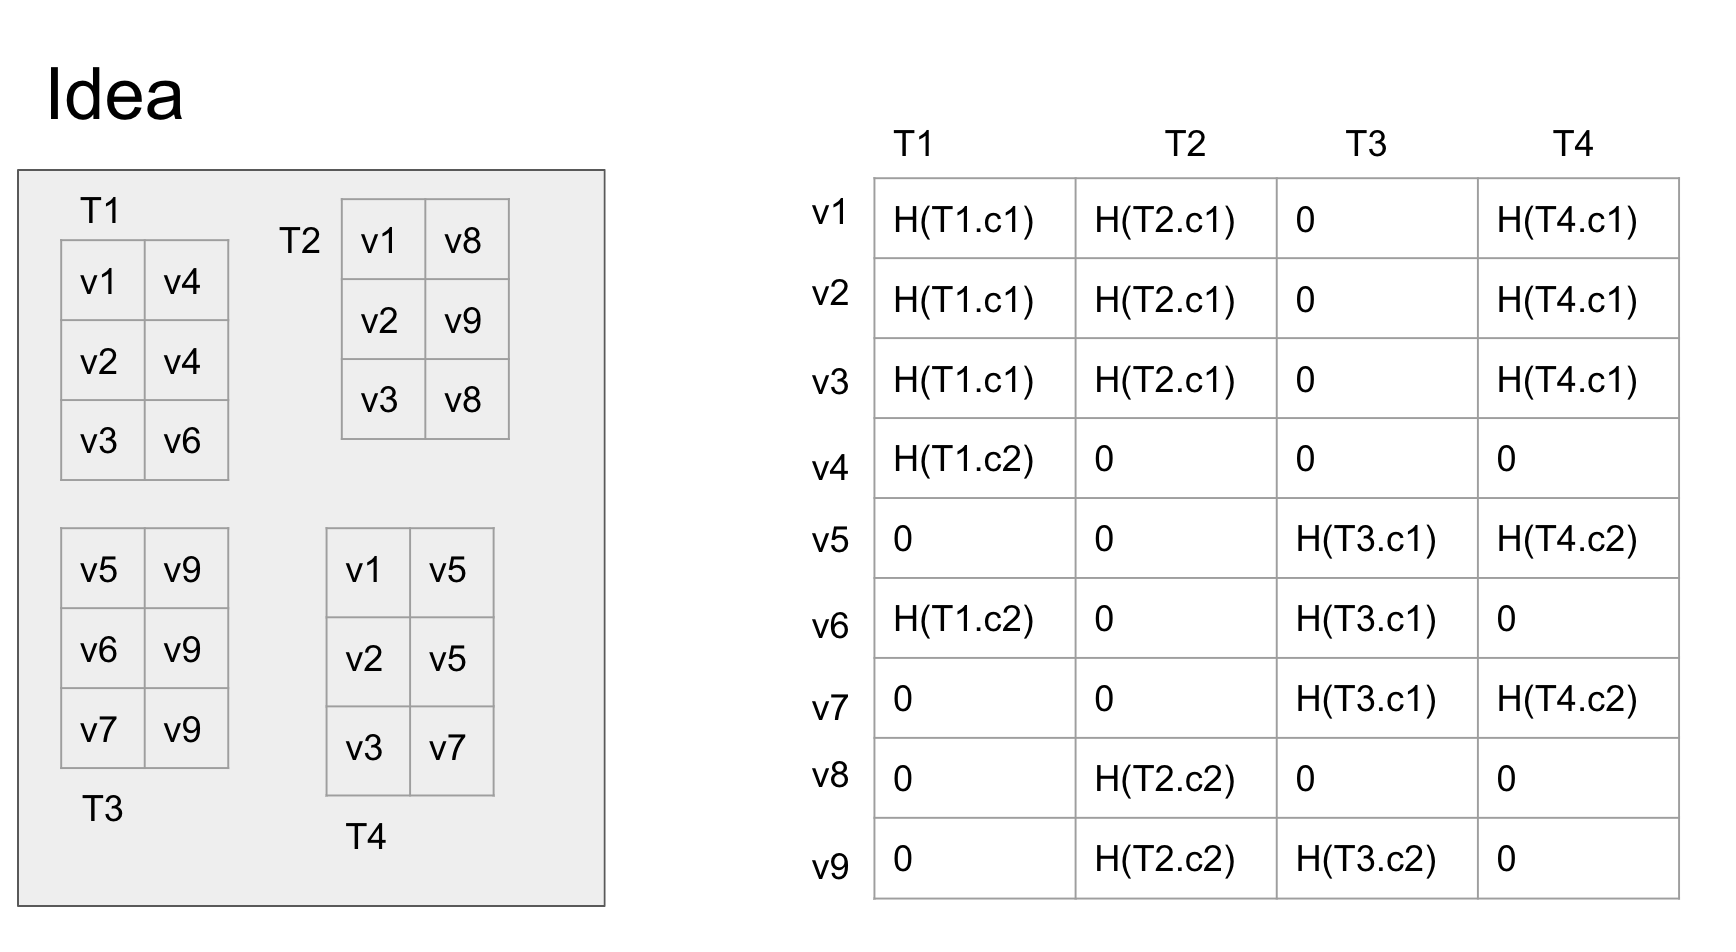
\includegraphics[scale=0.4]{figures/index_sketch.png}
    \caption{Sketch of entropy-based index for open data. When a value $v$ is present in column $j$ of table $i$, in postition $(v,j)$ it is stored the entropy of the column of $j$ of table $i$.}
\end{figure}

\begin{enumerate}
    \item We have analyze the state of the art approaches related to (i) open data searching and indexing, (ii) information-theoric measures sketching and (iii) information-theoric measures approximations. We found out that existing searching frameworks on open data only cares about finding the best, or the best k-set, of \textit{joining} tables or columns. This have many drawbacks, first of which the fact that the best join does not say anything about the best augmentation. For instance, the best join that a table can have is with itself, meaning a void augmentation. 
    \item We also noticed that there are information-theoretic measures that are particularly suitable in representing, or at least approximating, the behavior of functional dependencies. In particular, the conditional entropy $H(Y|X) = H(X)-I(X,Y)$, where $H(X)$ in the Shannon entropy of variable $X$ and $I(X,Y)$ is the mutual information between variables $X$ and $Y$, has lower bound 0 and upper bound $H(X)$. These two cases coincides with full functional dependency\footnote{Note that, despite the differentiation that we made in Section \ref{related} about functional dependency, up to now the interpretation is the same on classical database FDs and descriptive FDs.} when $H(Y|X) = 0$ (meaning that the value of $Y$ is totally determined by $X$) and complete independence, when $H(Y|X) = H(Y)$ (meaning that the knowledge of variable $X$ has no impact on the knowledge of $X$). This observation, mixed with the intuition that if a functional dependency (in its descriptive interpretation) between a set of attributes and a specific target holds these attributes are interesting for the augmentation, means that discovering FDs that minimize the conditional entropy\footnote{Acutally, our intuition derived by the fraction of information, i.e., a normalized variant of the mutual information. However, it is possible to show that minimizing the conditional entropy is equal to maximize the fraction of information.} produce the best augmentation. However, the approach of identifying a target attribute and discover FDs in such a way requires the materialization of the join, that as discussed in Section \ref{related} is unfeasible on data lakes.
    \item To overcome the issue of the join materialization, we decided to exploit the idea of an inverted index, in which the information of each table is stored, along with each column entropy and the association column-table. The peculiarity of this index is that it looks like a sparse matrix, since all the unique values in all the tables are indexed, and the entropy information for each column is stored only when i-th values belongs to j-th column. Figure \ref{index_sketch} shows a sketch of the designed index.
    \item We are currently working on the implementation of such an index, along with the research for understanding if mixing up the entropies is enough to simulate the conditional entropy behavior or a bit more elaborated metrics is required.
\end{enumerate}


